\section{ФУНКЦИОНАЛЬНОЕ ПРОЕКТИРОВАНИЕ}
\label{sec:functional}
Ниже будет описана работа разрабатываемого проекта и представлена информация о структуре программного продукта.

В проекте использован объектно-ориентированный подход, поэтому код проекта разделён на классы. Каждый класс выполняет свою уникальную функцию или расширяет функционал, предоставляемый фреймворком и сторонними библиотеками. Для взаимодействия всех классов и для интеграции проекта с дополнительными библиотеками используются файлы конфигурации.

Так же, так как сбор статистики и анализ тональностей --- независимые друг от друга задачи, то проект представляет собой два приложения, управляемые внешним скриптом.
\subsection{Структура проекта}
Разрабатываемый проект разделен на несколько каталогов:
\begin{itemize}
\item data\_gather --- хранит код сбора данных;
\item sentiment --- хранит код анализатора тональностей;
\item data --- хранит временные данные программы и входные данные;
\item javascript --- хранит код модуля визуализации;
\item treebank --- хранит код скриптов предобработки наборов данных.
\end{itemize}
\subsection{Структура базы данных}
Модель данных, иллюстрирующая таблицы базы данных и связи между ними приведена на чертеже ГУИР.400201.009 РР.3. В качестве базы данных была использована MySQL\@. Как видно из чертежа, для реализации связей один ко многим были использованы удаленные ключи, а для реализации связей много ко многим были созданы ассоциативные таблицы.
\subsection{Объектно-реляционное отображение}
В Python существует возможность не обращаться на прямую к базе данных. Это можно сделать при помощи \texttt{Sqlalchemy} --- инструмента объектно-реляционного отображения. \texttt{Sqlalchemy} предоставляет удобный функционал для работы с базами данных. В программной модели создается класс, соответствующий какой-то таблице из модели данных, и наследуется от класса \texttt{sqlalchemy.Model}. Используя магическое поле \texttt{\_\_tablename\_\_} указывается таблица, которой соответствует данный класс. Затем задаются поля класса, соответствующие столбцам таблицы базы данных, инстанцированные от класса \texttt{sqlalchemy.Column}. Так же указывается тип данных, который столбец имеет в базе данных. Затем описываются отношения с другими таблицами. Для этого предназначен модуль \texttt{sqlalchemy.orm}. С помощью функции \texttt{relationship} данного модуля можно задать простую связь, соответствующую удаленному ключу в базе данных. Существуют так же инструменты для реализации более сложных видов связей, вроде ассоциативных таблиц. Однако, инструмент ассоциативных таблиц не был использован в объектно-реляционном отображении в данном проекте, несмотря на то что данные таблицы широко используются в проекте для реализации связей вида много ко многим.

Пример объектно-реляционного отображения таблицы \texttt{item} показан ниже:

\medskip
\begin{lstlisting}[style=Python]
class Item(Base, DeclarativeBase):
    """The model for Item data"""
    __tablename__ = "item"

    id = sa.Column(sa.Integer, primary_key=True)
    name = sa.Column(VARCHAR(100, charset='utf8'), unique=True)
    cost = sa.Column(sa.Integer, primary_key=True)
    rating = sa.Column(sa.Integer, primary_key=True)
    state = sa.Column(VARCHAR(100, charset='utf8'), unique=True)
    number = sa.Column(sa.Integer, primary_key=True)
    sold = sa.Column(sa.Integer, primary_key=True)

    seller = orm.relationship("Seller", back_populates="items")
    store = orm.relationship("Store", back_populates="items")
\end{lstlisting}
\medskip

Как видно из приведенной на чертеже ГУИР.400201.009 РР.1 диаграммы классов, все таблицы модели данных имеют соответствующий класс в программной модели.

Класс \texttt{models.Category} представляет категорию товаров онлайн магазина. Имеет два публичных поля: \texttt{id} типа \texttt{sqlalchemy.Integer} и \texttt{name} типа \texttt{sqlalchemy.String} хранящие соответственно идентификатор в базе данных и название категории.

Класс \texttt{models.ItemSubCategory} представляет подкатегорию товара в онлайн магазине. Публичные поля \texttt{id} типа \texttt{sqlalchemy.Integer}, \texttt{name} типа \texttt{sqlalchemy.String} и \texttt{category} типа \texttt{models.Category} хранят соответственно идентификатор в базе данных, название подкатегории и сслыку на объект категории, к которой данная подкатегория принадлежит. Так как подкатегория --- это составная часть категории, то при удалении объекта категории должен удаляться и объект подкатегории, на который ссылается объект категории, то между классами \texttt{models.ItemSubCategory} и \texttt{models.Category} устанавливается связь типа композиции, направленная от подкатегории к категории, как видно из приведенной на чертеже ГУИР.400201.009 РР.1 диаграммы классов.

Класс \texttt{models.CategoryLink} представляет ассоциативную таблицу для связи товара с его подкатегорией. Так как каждый товар может состоять в произвольном количестве подкатегорий, а подкатегория может содержать произвольное количество товаров, то между ними связь вида много ко многим. Таким образом, каждый объект класса данной ассоциативной таблицы представляет связь между объектом подкатегории и объектом товара. Публичное поле \texttt{sub\_category} типа \texttt{models.ItemSubCatego\-ry} класса \texttt{mo\-dels.CategoryLink} хранит ссылку на объект класса подкатегории. При удалении подкатегории свзяь так же должна разрушаться. Поэтому из класса ассоциативной таблицы \texttt{models.CategoryLink} исходит отношение вида композиция в сторону класса подкатегории \texttt{models.Item\-Sub\-Ca\-te\-go\-ry}, что видно из диаграммы классов на чертеже ГУИР.400201.009.РР1.1. Также \texttt{models.Cate\-goryLink} хранит ссылку на объект товара в публичном поле \texttt{item} типа \texttt{mo\-dels.Item}. Так как при разрушении объекта товара связь между товаром и подкатегорией теряет смысл, то объект типа \texttt{models.} \texttt{Ca\-te\-go\-ry\-Link} также должен быть уничтожен. Таким образом от класса ассоциативной таблицы \texttt{mo\-dels.} \texttt{CategoryLink} исходит связь типа композиции в сторону класса товара \texttt{Item}. Данная композиция отражена на диаграмме классов, изображенной на чертеже ГУИР.400201.009.РР.1.

Следующие классы являются объектно-реляционными отображениями:
\begin{itemize}
\item \texttt{models.Category};
\item \texttt{models.ItemSubCategory};
\item \texttt{models.CategoryLink};
\item \texttt{models.Item};
\item \texttt{models.Store};
\item \texttt{models.AchievementLink};
\item \texttt{models.Achievement};
\item \texttt{models.Seller};
\item \texttt{models.User};
\item \texttt{models.SellerReview};
\item \texttt{models.ItemReview};
\item \texttt{models.Tree};
\item \texttt{models.Treebank};
\item \texttt{models.Genre};
\item \texttt{models.GenreLink};
\item \texttt{models.Actor};
\item \texttt{models.ActorLink};
\item \texttt{models.Director};
\item \texttt{models.DirectorLink};
\item \texttt{models.Film};
\item \texttt{models.FilmReviewAuthor};
\item \texttt{models.FilmReview}.
\end{itemize}

Класс \texttt{models.Item} представляет товар интернет магазина. Публичные поля \texttt{id} типа \texttt{sqlalchemy.Integer} и \texttt{name} типа \texttt{sqlalchemy.String} хранят соответственно идентификатор в базе данных и наименование товара. Далее поля \texttt{cost} типа \texttt{sqlalchemy.Integer}, \texttt{rating} типа \texttt{sqlalchemy.Integer}, \texttt{state} типа \texttt{sqlalchemy.String}, \texttt{number} типа \texttt{sqlalchemy.Integer} и \texttt{sold} типа \texttt{sqlalchemy.Integer} хранят соответственно цену товара, рейтинг товара, состояние, количество товара в наличии и товара продано. Затем два поля \texttt{seller} типа \texttt{models.Seller} и \texttt{store} типа \texttt{models.Store} хранят ссылки на объекты продавца и магазина соответственно.

Класс \texttt{models.Store} представляет магазин интернет площадки. Имеет два публичных поля: \texttt{id} типа \texttt{sqlalchemy.Integer} и \texttt{name} типа \texttt{sqlal\-chemy.String} хранящие соответственно идентификатор в базе данных и название магазина. Так как магазин является лишь композицей для товаров, то товар может существовать без магазина, верно и обратное --- магазин может существовать без товара. Поэтому между классами товара \texttt{models.Item} и магазина \texttt{models.Store} образована свзяь типа агрегация, как это видно из диаграммы классов на чертеже ГУИР.400201.009.РР.1.

Класс \texttt{models.Achievement} представляет собой достижение магазина интернет площадки. Публичные поля \texttt{id} типа \texttt{sqlalchemy.Integer} и \texttt{name} типа \texttt{sqlalchemy.String} хранят соответственно идентификатор в базе данных и название достижения.

Так как каждый магазин может иметь произвольное количество достижений, а каждое достижение может принадлежать нескольким магазинам, то между достижением и магазином связь много ко многим. Поэтому класс \texttt{models.AchievementLink} представляет собой ассоциативную таблицу, а какждый объект данного типа будет представлять связь между объектом достижения и объектом магазина. Класс \texttt{models.AchievementLink} имеет публичное поле \texttt{achievement} типа \texttt{models.Achievement}, которое хранит ссылку на объект класса достижения. При удалении достижения свзяь между достижением и магазином так же должна разрушаться. Поэтому из класса ассоциативной таблицы \texttt{models.AchievementLink} исходит связь вида композиция в сторону класса достижения \texttt{models.Achievement}, что отображено на диаграмме классов, изображенной на чертеже ГУИР.400201.009.РР.1. Также \texttt{models.AchievementLink} хранит ссылку на объект магазина в публичном поле \texttt{store} типа \texttt{models.Store}. Так как при разрушении объекта магазина связь между магазином и достижением теряет смысл, то объект типа \texttt{models.AchievementLink} также должен быть уничтожен. Таким образом от класса ассоциативной таблицы \texttt{models.AchievementLink} исходит связь типа композиции в сторону класса магазина \texttt{Store}. Данные композиция отражена на диаграмме классов на чертеже ГУИР.400201.009.РР.1.

Класс \texttt{models.Seller} представляет собой описание продавца интернет магазина. Публичные поля \texttt{id} типа \texttt{sqlalchemy.Integer} и \texttt{name} типа \texttt{sqlal\-chemy.String} хранят соответственно идентификатор в базе данных и логин продавца. Так же он имеет поля \texttt{description\_rating} типа \texttt{sqlalchemy.In\-teger}, \texttt{communication\_rating} типа \texttt{sqlalchemy.Integer}, \texttt{timing\_rating} типа \texttt{sqlalchemy.Integer} и \texttt{delivery\_cost\_rating} типа \texttt{sqlalchemy.Integer} которые хранят соответственно рейтинги продавца по следующим параметрам:
\begin{itemize}
\item рейтинг точности составления описания;
\item рейтинг общения с продавцом;
\item рейтинг своевременности доставки;
\item рейтинг удовлетворенностью ценой доставки.
\end{itemize}
При удалении товара объект продавца должен быть сохранен. А при удалении объекта продавца объект товара должен быть сохранен. Но так как объект товара имеет ссылку на продавца, то от класса \texttt{models.Item} направлена связь типа агрегация в сторону класса \texttt{models.Seller}. Связь отражена на диаграмме классов, изображенной на чертеже ГУИР.400201.009.РР.1. Также, класс \texttt{models.Store} связан с классом \texttt{models.Seller} отношением типа ассоциация, из-за того, что между ними может существовать косвенная связь, вплоть до того, что продавец и магазин будут отражать один и тот же объект. То есть продавец может оказаться частью магазина в модели интернет площадки, а может быть и самостоятельным объектом.

Класс \texttt{models.User} представляет объект пользователя. Идентификатор объекта в базе данных и логин пользователя хранятся соответственно в полях \texttt{id} типа \texttt{sqlalchemy.Integer} и \texttt{login} типа \texttt{sqlalchemy.String}. Публичные поля \texttt{addres} типа \texttt{sqlalchemy.String}, \texttt{country} типа \texttt{sqlalchemy.String}, \texttt{sta\-te} типа \texttt{sqlalchemy.String}, \texttt{rating} типа \texttt{sqlalchemy.Integer} и \texttt{birth\_date} типа \texttt{sqlalchemy.Date} хранят соответственно адрес доставки пользователя, страна, время последнего выхода в онлайн, рейтинг пользователя и дата рождения.

Класс \texttt{models.Genre} представляет жанр фильма на форуме о кино. Имеет два публичных поля: \texttt{id} типа \texttt{sqlalchemy.Integer} и \texttt{name} типа \texttt{sqlalche\-my.String} хранящие соответственно идентификатор в базе данных и название жанра кино.

Класс \texttt{models.SellerReview} представляет обзор на продавца в интернет магазине. Публичные поля \texttt{id} типа \texttt{sqlalchemy.Integer} и \texttt{review\_text} типа \texttt{sqlalchemy.String} хранят соответственно идентификатор в базе данных и текст отзыва на продавца. Оценка продавца пользователем хранится в публичном поле \texttt{seller\_grade} типа \texttt{sqlalchemy.Integer}. Автор отзыва указан ссылкой на объект пользователя в публичном поле \texttt{user} типа \texttt{models.User}. Так как при удалении пользователя, обзор теряет силу и значимость, то необходимо удалять вслед за этим и объект обзора на продавца в интернет магазине. Таким образом от класса обзора \texttt{models.SellerReview} направлена связь вида композиция в сторону класса \texttt{models.User}. Композиция отражена в диаграмме классов, изображенной на чертеже ГУИР.400201.009.РР.1. В поле \texttt{seller} типа \texttt{models.Seller} хранится ссылка на объект продавца интернет магазина, описанного в данном объекте отзыва. При удалении объекта продавца, который описывает текущий объект отзыва на продавца, отзыв на продавца так же должен быть удален. Следовательно, от класса отзыва \texttt{models.SellerReview} направлена связь типа композиция в сторону класса продавца \texttt{models.Seller}. Данная композиция также отражена на диаграмме классов на чертеже ГУИР.400201.009.РР.1. Также класс \texttt{models.SellerRevi\-ew} хранит ссылку на объект синтаксического дерева, в публичном поле \texttt{tree} типа \texttt{models.Tree}. Так как объект синтаксического дерева хранит текст отзыва на продавца в интернет магазине в формате синтаксического дерева, то при удалении объекта отзыва на продавца, объект синтаксического дерева должен быть так же удален. Значит, от класса продавца \texttt{models.Seller} направлена связь типа композиция в сторону класса обзора \texttt{models.SellerReview}. Данная связь также отражена в диаграмме классов, изображенной на чертеже ГУИР.400201.009.РР.1.

Так как каждый фильм может принадлежать к произвольному количеству жанров, а каждый жанр может быть присвоен нескольким фильмам, то между жанром и фильмом связь много ко многим. Поэтому класс \texttt{models.Gen\-reLink} представляет собой ассоциативную таблицу, а какждый объект данного типа будет представлять связь между объектом жанра и объектом фильма. Класс \texttt{models.GenreLink} имеет публичное поле \texttt{genre} типа \texttt{models.Gen\-re}, которое хранит ссылку на объект класса жанра кино на тематическом форуме. При удалении жанра свзяь между жанром и фильмом так же должна разрушаться. Поэтому из класса ассоциативной таблицы \texttt{models.GenreLink} исходит связь вида композиция в сторону класса жанра \texttt{models.Genre}. Данная связь отражена на диаграмме классов чертеже ГУИР.400201.009.РР.1. Также \texttt{models.GenreLink} хранит ссылку на объект фильма в публичном поле \texttt{film} типа \texttt{models.Film}. Так как при разрушении объекта фильма связь между фильмом и жанром фильма теряет смысл, то объект типа \texttt{models.GenreLink} также должен быть уничтожен. Таким образом от класса ассоциативной таблицы \texttt{models.GenreLink} исходит связь типа композиции в сторону класса фильма \texttt{models.Film}. Данная связь также отражена диаграмме классов, изображенной на чертеже ГУИР.400201.009.РР.1.

Класс \texttt{models.Film} представляет собой объект фильма на тематическом форуме. Публичные поля \texttt{id} типа \texttt{sqlalchemy.Integer} и \texttt{title} типа \texttt{sqlalchemy.String} хранят соответственно идентификатор в базе данных и название фильма. Информация о дате выхода фильма прокат в кинотеатрах, страна производства фильма и бдюжет хранится соответственно в полях: \texttt{year} типа \texttt{sqlal\-chemy.Date}, \texttt{country} типа \texttt{sqlalchemy.String} и \texttt{budget} типа \texttt{sql\-alchey.Integer}.

Класс \texttt{models.Filmreviewauthor} представляет автора отзыва на фильм на тематическом форуме. Имеет два публичных поля: \texttt{id} типа \texttt{sqlalchemy.In\-teger} и \texttt{name} типа \texttt{sqlalchemy.String} хранящие соответственно идентификатор в базе данных и имя автора отзыва на фильм на тематическом форуме.

Класс \texttt{models.FilmReview} представляет обзор на фильм на таматическом форуме. Публичные поля \texttt{id} типа \texttt{sqlalchemy.Integer} и \texttt{name} типа \texttt{sql\-alchemy.String} хранят соответственно идентификатор в базе данных и текст отзыва на фильм. Оценка фильма пользователем хранится в публичном поле \texttt{film\_grade} типа \texttt{sqlalchemy.Integer}. Автор отзыва указан ссылкой на объект автора в публичном поле \texttt{authpr} типа \texttt{models.FilmReviewAuthor}. Так как обзор должен иметь автора, то при удалении автора необходимо удалять вслед за этим и объект обзора на фильм. Таким образом от класса \texttt{models.Fi\-lmReview} направлена связь вида композиция в сторону класса \texttt{models.Film\-ReviewAuthor}, что видно из диаграммы классов на чертеже ГУИР.400201.0\-09.РР.1. В поле \texttt{film} типа \texttt{models.Film} хранится ссылка на объект фильма, описанного в данном объекте отзыва. При удалении объекта фильма, который описывает текущий объект отзыва на фильм, то отзыв на фильм так же должен быть удален. Следовательно, от класса \texttt{models.ItemFilm} направлена связь типа композиция в сторону класса \texttt{models.Film}. Данная композиция изображена на диаграмме классов на чертеже ГУИР.400201.009.РР.1. Также \texttt{models.FilmReview} хранит ссылку на объект синтаксического дерева, в публичном поле \texttt{tree} типа \texttt{models.Tree}. Так как объект синтаксического дерева хранит текст отзыва на фильм в формате синтаксического дерева, то при удалении объекта отзыва на фильм, объект синтаксического дерева должен быть так же удален. Значит, от класса \texttt{models.Tree} направлена связь типа композиция в сторону класса \texttt{models.FilmReview}. Данная связь отражена на диаграмме классов, изображенной на чертеже ГУИР.400201.009.РР.1.

Класс \texttt{models.Actor} представляет актера кино на тематическом форуме. Имеет два публичных поля: \texttt{id} типа \texttt{sqlalchemy.Integer} и \texttt{name} типа \texttt{sqlalchemy.String} хранящие соответственно идентификатор в базе данных и имя актера.

Так как в каждом фильме может сниматься произвольное количество актеров, а каждый актер может играть роли в произвольном количестве фильмов, то между актером и фильмом связь много ко многим. Поэтому класс \texttt{models.ActorLink} представляет собой ассоциативную таблицу, а какждый объект данного типа будет представлять связь между объектом фильма и объектом актера. Класс \texttt{models.ActorLink} имеет публичное поле \texttt{actor} типа \texttt{models.Actor}, которое хранит ссылку на объект класса актера кино на тематическом форуме. При удалении актера свзяь между актером и фильмом так же должна разрушаться. Поэтому из класса ассоциативной таблицы \texttt{models.\-ActorLink} исходит связь вида композиция в сторону класса актера \texttt{models.\-Actor}. Данная связь отражена на диаграмме классов, изображенной на чертеже ГУИР.400201.009.РР.1. Также \texttt{models.ActorLink} хранит ссылку на объект фильма в публичном поле \texttt{film} типа \texttt{models.Film}. Так как при разрушении объекта фильма связь между фильмом и актером теряет смысл, то объект типа \texttt{models.ActorLink} также должен быть уничтожен. Таким образом от класса ассоциативной таблицы \texttt{models.ActorLink} исходит связь типа композиции в сторону класса фильма \texttt{models.Film}. Данная связь также отражена на диаграмме классов, изображенной на чертеже ГУИР.400201.009.РР.1.

Класс \texttt{models.Treebank} представляет собой отображение набора синтаксических деревьев, хранящихся в базе данных. Имеет два публичных поля: \texttt{id} типа \texttt{sqlalchemy.Integer} и \texttt{name} типа \texttt{sqlalchemy.String} хранящие соответственно идентификатор в базе данных и название набора данных. Название набора данных выбирается одно из ряда:
\begin{itemize}
\item \texttt{sst\_dev};
\item \texttt{sst\_test};
\item \texttt{sst\_train};
\item \texttt{film\_reviews};
\item \texttt{item\_reviews};
\item \texttt{seller\_reviews}.
\end{itemize}
Код \texttt{sst} обозначает Stanford Sentiment Treebank --- Стенфордский набор данных. Так же в базе хранятся наборы данных созданные из обзоров на фильмы, полученные из тематического форума --- \texttt{film\_reviews}, из онлайн магазина --- \texttt{item\_reviews}, и также обзоры на продавцов --- \texttt{seller\_reviews}.

Класс \texttt{models.ItemReview} представляет обзор на товар в интернет магазине. Публичные поля \texttt{id} типа \texttt{sqlalchemy.Integer} и \texttt{review\_text} типа \texttt{sqlalchemy.String} хранят соответственно идентификатор в базе данных и текст отзыва на товар. Оценка товара пользователем хранится в публичном поле \texttt{item\_grade} типа \texttt{sqlalchemy.Integer}. Автор отзыва указан ссылкой на объект пользователя в публичном поле \texttt{user} типа \texttt{models.User}. Так как при удалении пользователя, обзор теряет силу и значимость, то необходимо удалять вслед за этим и объект обзора на товар. Таким образом от класса \texttt{models.ItemReview} направлена связь вида композиция в сторону класса \texttt{models.User}, что отображено на диаграмме классов, изображенной на чертеже ГУИР.400201.009.РР.1. В поле \texttt{item} типа \texttt{models.Item} хранится ссылка на объект товара, описанного в данном объекте отзыва. При удалении объекта товара, который описывает текущий объект отзыва на товар, отзыв на товар в интернет магазине так же должен быть удален. Следовательно, от класса \texttt{models.ItemReview} направлена связь типа композиция в сторону класса \texttt{models.Item}. Данная композиция изображена на диаграмме классов на чертеже ГУИР.400201.009.РР.1. Также класс \texttt{models.ItemReview} хранит ссылку на объект синтаксического дерева в публичном поле \texttt{tree} типа \texttt{models.Tree}. Так как объект синтаксического дерева хранит текст отзыва в формате синтаксического дерева, то при удалении объекта отзыва на товар в интернет магазине, объект синтаксического дерева должен быть так же удален. Значит, от класса \texttt{models.Tree} направлена связь типа композиция в сторону класса \texttt{models.ItemReview}. Данная композиция также отображена на диаграмме классов, изображенной на чертеже ГУИР.400201.009.РР.1.

Класс \texttt{models.Director} представляет режиссера кино на тематическом форуме. Имеет два публичных поля: \texttt{id} типа \texttt{sqlalchemy.Integer} и \texttt{name} типа \texttt{sqlalchemy.String} хранящие соответственно идентификатор в базе данных и имя режиссера.

Так как в каждом фильме может участвовать произвольное количество режиссеров, а каждый режиссер может снимать произвольное количество фильмов, то между режиссером и фильмом связь много ко многим. Поэтому класс \texttt{models.DiretorLink} представляет собой ассоциативную таблицу, а какждый объект данного типа будет представлять связь между объектом фильма и объектом режиссера. Класс \texttt{models.DirectorLink} имеет публичное поле \texttt{director} типа \texttt{models.Director}, которое хранит ссылку на объект класса режиссера кино на тематическом форуме. При удалении режиссера свзяь между режиссером и фильмом так же должна разрушаться. Поэтому из класса ассоциативной таблицы \texttt{models.DirectorLink} исходит связь вида композиция в сторону класса режиссера \texttt{models.Director}. Данная связь отражена на диаграмме классов на чертеже ГУИР.400201.009.РР.1. Также \texttt{models.Di\-rectorLink} хранит ссылку на объект фильма в публичном поле \texttt{film} типа \texttt{models.Film}. Так как при разрушении объекта фильма связь между фильмом и его режиссером теряет смысл, то объект типа \texttt{models.DirectorLink} также должен быть уничтожен. Таким образом от класса ассоциативной таблицы \texttt{models.DirectorLink} исходит связь типа композиции в сторону класса фильма \texttt{models.Film}. Данная композиция также отражена на диаграмме классов, изображенной на чертеже ГУИР.400201.009.РР.1.

Класс \texttt{models.Tree} представляет объект синтаксического дерева. Публичные поля \texttt{id} типа \texttt{sqlalchemy.Integer} и \texttt{json} типа \texttt{sqlalchemy.String} хранят соответственно идентификатор в базе данных и представление синтаксического дерева в формате JSON\@. Поле \texttt{treebank} типа \texttt{models.Treebank} хранит ссылку на объект набора данных. Так как синтаксическое дерево может быть независимым и не входить ни в один из наборов данных, но иимеет поле ссылки на \texttt{models.Treebank}, то между классами набора данных и синтаксического дерева создается связь вида агрегация направленная он \texttt{mo\-dels.Tree} в сторону \texttt{models.Treebank}. Данная агрегация отображена на диаграмме классов на чертеже ГУИР.400201.009.РР.1.
\subsection{Модуль сбора статистики}
Модуль сбора статистики, описанный в downloader.py в виде класса Downloader, осуществляет сбор статистики с интернет ресурсов, и сохраняет её в базе данных. Для работы с базой класс имеет поля \texttt{session} типа \texttt{sqlalchemy.Session} и \texttt{db\_driver} типа \texttt{sqlalchemy.DbDriver}. В объекте \texttt{db\_driver} содержится информация о подключении к базе данных:
\begin{itemize}
\item база данных (MySQL\@ или PostgreSQL\@)
\item драйвер базы данных для \texttt{Python} (напрмер \texttt{oursql} или \texttt{pymysql})
\item адрес хоста базы;
\item имя базы;
\item логин;
\item пароль.
\end{itemize}
Далее он имеет конфигурируемые переменные \texttt{FILM\_TOKEN\_LEN} и \texttt{ITEM\_TO\-KEN\_LEN}, заданные глобально в модуле Python. Это стандартная практика для защиты конфигурации. Данные переменные задают количество скачиваемых объектов за один REST запрос для фильмов и товаров соответственно. В константах \texttt{STORE\_URL} и \texttt{FILM\_FORUM\_URL} хранятся URL целевых ресурсов. Массивы \texttt{item\_reviews}, \texttt{seller\_reviews} и \texttt{film\_reviews} хранят соответственно объекты реляционного отображения таблиц с отзывами.

Класс \texttt{Downloader} содежрит набор схожих методов:
\begin{itemize}
\item \texttt{get\_items};
\item \texttt{get\_film};
\item \texttt{get\_categories};
\item \texttt{get\_stores};
\item \texttt{get\_sellers};
\item \texttt{get\_achivements};
\item \texttt{get\_actors};
\item \texttt{get\_directors};
\item \texttt{get\_subcategories}.
\end{itemize}

Задача данных методов в том, чтобы преобразовать полученный от интернет ресурса GET ответ в формате JSON в объек объектно реляциоонного отображения, создав тем самым соответствующую запись в базе данных. Каждый из этих методов имеет константу, хранящую часть путь в URL адресе. Далее имеется переменная {\texttt{params}} типа \texttt{dict}, хранящая параметры REST запросов. Пример объявления \texttt{params} показан ниже:

\medskip
\begin{lstlisting}[style=Python]
  params = {'sortBy': 'recentlyCreated',
    'group': 'general',
    'page': 1,
    'pageSize': self.FILM_PAGE_SIZE}
\end{lstlisting}
\medskip

Переменная \texttt{response} типа хранит ответы на REST запросы. Так же множество различных локальных переменных введены для хранения промежуточных результатов преобразования из JSON в объект. Методы \texttt{save\_fi\-lm\_info} и \texttt{save\_item\_info} формируют конечную транзацкию в базу данных.

Наконец, задача метода \texttt{get\_missing} проверить целостность данных в базе. Для этого используется схожий набор переменных: \texttt{params} и \texttt{response} для управления REST запросами. Для проверки целостности со стороны клиента используются массивы класса \texttt{item\_reviews}, \texttt{seller\_reviews} и \texttt{film\_\-reviews}.
\subsection{Модуль ячейки Tree LSTM}
Класс \texttt{cstlstm.ChildSumTreeLSTMCell} выделен в модуль ячейки Tree LSTM за счет его математической сложности. Класс имеет следующие поля:
\begin{itemize}
\item \texttt{unit\_number};
\item \texttt{forget\_bias};
\item \texttt{forget\_signals};
\item \texttt{iou\_signals};
\item \texttt{input\_transform}.
\end{itemize}

Публичное поле \texttt{unit\_number} имеет тип \texttt{int}. Хранит количество нейронов скрытого слоя нейронной сети в архитектуре Child-Sum Tree LSTM\@. Далее, публичное поле \texttt{forget\_bias} типа \texttt{float} содержит $b^{(f)}$ применяющийся в формуле~\ref{eq:func:lstm:forget}. Публичное поле \texttt{forget\_signals} типа \texttt{keras.Layers.Dense} описывает само уравнение~\ref{eq:func:lstm:forget}. \texttt{keras.Layers.Dense} является реализацией базового слоя нейронной сети. В данном слое будут две обучаемые переменные: матрица весов и вектор сдвига. Они соответствуют членам формулы $W^{(f)}$, $U^{(f)}$ и $b^{(f)}$. Класс \texttt{keras.Layers.Dense} поддерживает автоматическое вычисление градиента и оптимизацию обучаемых переменных. Публичное поле \texttt{iou\_signals} типа \texttt{keras.Layers.Dense} выполняет схожую функцию для одновременного вычисления сигналов, описанных формулами~\ref{eq:func:lstm:i},~\ref{eq:func:lstm:o} и~\ref{eq:func:lstm:u}.

Последнее публичное поле \texttt{input\_transform} типа \texttt{keras.Layers.Den\-se} реализует~\ref{eq:func:lstm:transform}.

Код инициализации класса \texttt{cstlstm.ChildSumTreeLSTMCell} представлен в листинге ниже:

\medskip
\begin{lstlisting}[style=Python]
  def __init__(self, unit_number, reg_factor, forget_bias=1.0):
    super(ChildSumTreeLSTMCell, self).__init__()
    self.unit_number = unit_number
    self.forget_bias = forget_bias
    self.forget_signals = layers.Dense(unit_number, input_shape=(300 + unit_number,), kernel_regularizer=tf.keras.regularizers.l2(reg_factor))
    self.iou_signals = layers.Dense(unit_number * 3, kernel_regularizer=tf.keras.regularizers.l2(reg_factor))
    self.input_transform = layers.Dense(unit_number, kernel_regularizer=tf.keras.regularizers.l2(reg_factor))
\end{lstlisting}
\medskip

Входной параметр конструктора класса \texttt{cstlstm.ChildSumTreeLSTM\-Cell} \texttt{reg\_factor} --- коэффициент регуляризации L2. Как видно в листинге, полносвязные слои, такие как \texttt{forget\_signals}, \texttt{iou\_signals} и \texttt{input\_trans\-form}, в качестве параметра конструктора получают также объект типа \texttt{ke\-ras.regularizers.l2}. Данный параметр задаст регуляризацию L2, для того чтобы смесить математическое ожидание ближе к верному предсказанию за счет увеличения дисперсии.

Класс \texttt{cstlstm.ChildSumTreeLSTMCell} имеет только один метод \texttt{call (self, inputs, *args, **kwargs)}. Это переопределенный метод класса \texttt{keras.Layers.Model}. Данный метод вызывается, когда проиходит обращение к объекту типа \texttt{keras.Layers.Model} в ходе выполнения графа обработки Tensorflow. Параметр \texttt{inputs} типа \texttt{tensorflow.Tensor} содержит входные данные в виде многомерного массива. Задача метода в том, чтобы обработать входной тензор согласно логике слоя Child-Sum Tree LSTM и затем вернуть результат в формате \texttt{tensorflow.Tensor}.

\subsection{Модуль анализатора и модуль выделения особенностей}
В модуль анализатора включены следующие классы:
\begin{itemize}
\item \texttt{cstlstm.ChildSumTreeLSTMClassifier};
\item \texttt{train.Train};
\item \texttt{train.Treebank};
\item \texttt{inference.Inference}.
\end{itemize}
Их задача в том, чтобы обучать модель Child-Sum Tree LSTM, и делать предсказания тональностей для некоторых наборов данных. Модуль выделения особееностей включен в классы модуля анализатора в качетсве модели встраивания слов GloVe, что будет расмотрено далее.

Класс \texttt{cstlstm.ChildSumTreeLSTMClassifier} реализует архитектуру Child-Sum Tree LSTM\@. Данный класс обладает следующими публичными полями:
\begin{itemize}
\item \texttt{embed};
\item \texttt{projection};
\item \texttt{encoder};
\item \texttt{output\_layer};
\item \texttt{dropout};
\item \texttt{reg\_factor};
\item \texttt{loss};
\item \texttt{result};
\item \texttt{fine};
\item \texttt{binary};
\item \texttt{root\_fine};
\item \texttt{root\_binary}.
\end{itemize}

Публичное поле \texttt{embed} типа \texttt{tensorflow.Tensor} представляет собой матрицу встраивания слов.

Tensorflow --- это фреймворк, задача которого в, общем случае, упростить реализацию каких-то операций линейной алгебры, для выполнения их на графических процессорах, или тенсорных процессорах. Центральный процессор, и графический процессор или тенсорный процессор имеют раздельную память. Операции пересылки данных из памяти одного устройства в память другого довольно затратные и значительно замедляют результирующую производительность. Хотя в подавляющем большинстве случаев обращаются к выполнению вычислений на графических или тенсорных процессорах именно с целью повышения производительности алгоритма в сравнении с производительностью его выполнения на центральном процессоре. Поэтому, с целью сократить количество пересылок между устройствами памяти, фреймворки, созданные для реализации алгоритмов на графических процессорах, такие как Tensorflow или Theano, строят граф алгоритма, где четко заданы потоки перемещения и обработки данных.

Класс \texttt{tensorflow.Tensor} --- это бызовый класс Tensorflow, который представляет вывод какой-либо операции в графе выполнения алгоритма в Tensorflow. Объект типа \texttt{tenosorflow.Tensor} --- это символьный контроллер вывода операции, он не содержит самого численного результата выполнения операции. Но вместо этого он предоставляет возможность вычислить значение с помощью \texttt{tensorflow.Session}. У класса \texttt{tensorflow.Tenser} два основных предназначения:
\begin{itemize}
\item Объект \texttt{tensorflow.Tensor} может быть передан другой операции. Это создаст связь между операциями в графе выполнения Tensorflow.
\item После того как граф был запущен в \texttt{tensorflow.Session}, значение результата операции может быть получено с помощью \texttt{tensorflow.Sessi\-on.run}. \texttt{tensorflow.Tensor.eval()} --- это сокращение для \texttt{tensorflow.Ses\-sion.run()}
\end{itemize}

Публичное поле \texttt{embed} типа \texttt{tensorflow.Tensor} хранит константный двумерный массив, в каждой строке которой хранится некоторый вектор из модели GloVe.

Встраивание слов производится с помощью модели GloVe, которая обучена для кодировки семантики слов на основе контекста их использования. Однако, чтобы сделать модель более применимой для задачи классификации тональностей, её возможно дообучить. Продолжать тренировать модель GloVe одновременно с моделью Tree LSTM --- это крайне неэффективное решение, так как хотя бы сама модель в сжатом виде занимает 5 гигабайт дискового пространства. А вычисление градиента и последующая оптимизация такого количества векторов займет невероятно много времени. Поэтому оригинальная модель GloVe фильтруется. В ней оставляют только слова, использующиеся в тренировочном наборе данных. Отфильтрованная под Стенфордский набор синтаксических деревьев модель GloVe занимает уже 80 мегабайт дискового простанства. Затем, чтобы дообучать векторы из отфильтрованной модели GloVe, вводится ещё один слой нейронной сети. Это полносвязный слой, имеющий такое же количество нейронов, как и вектор GloVe. Таким образом, размерность векторов меняться не будет, однако их значение будет  оптимизироваться одновременно с параметрами всей архитектуры Child-Sum Tree LSTM во время процесса обучения. Задачу данного полносвязного слоя и выполняет публичное поле \texttt{projection} типа \texttt{keras.Layers.Dense} класса \texttt{cstlstm.ChildSumTreeLSTMClassifier}.

Конструктор класса \texttt{cstlstm.ChildSumTreeLSTMClassifier} представлен ниже:
\medskip
\begin{lstlisting}[style=Python]
  def __init__(self, embed, unit_numb=150, class_numb=5, reg_factor=0.0001, keep_prob=0.5):
    super(ChildSumTreeLSTMClassifier, self).__init__()
    self.embed = tf.constant(embed)
    self.projection = layers.Dense(self.embed.shape[1], kernel_regularizer=tf.keras.regularizers.l2(reg_factor))
    self.encoder = ChildSumTreeLSTMCell(unit_numb, reg_factor)
    self.output_layer = layers.Dense(class_numb, kernel_regularizer=tf.keras.regularizers.l2(reg_factor))
    self.dropout = layers.Dropout(keep_prob)
    self.reg_factor = reg_factor
    self.loss = 0
    self.result = []
    self.fine = tfe.metrics.Accuracy()
    self.binary = tfe.metrics.Accuracy()
    self.root_fine = tfe.metrics.Accuracy()
    self.root_binary = tfe.metrics.Accuracy()
    super(ChildSumTreeLSTMCell, self).__init__()
    self.unit_number = unit_number
    self.forget_bias = forget_bias
    self.forget_signals = layers.Dense(unit_number, input_shape=(300 + unit_number,), kernel_regularizer=tf.keras.regularizers.l2(reg_factor))
    self.iou_signals = layers.Dense(unit_number * 3, kernel_regularizer=tf.keras.regularizers.l2(reg_factor))
    self.input_transform = layers.Dense(unit_number, kernel_regularizer=tf.keras.regularizers.l2(reg_factor))
\end{lstlisting}
\medskip

Входные параметры конструктора класса \texttt{cstlstm.ChildSumTreeLSTM\-Classifier}:
\begin{itemize}
\item \texttt{embed};
\item \texttt{unit\_numb};
\item \texttt{class\_numb};
\item \texttt{reg\_factor};
\item \texttt{keep\_prob}.
\end{itemize}

Параметр \texttt{embed} типа \texttt{numpy.array} является матрицей плотных векторов модели GloVe. Остальные же параметры являются гиперпараметрами модели Child-Sum Tree LSTM\@. Параметр \texttt{unit\_numb} типа \texttt{int} задает количество нейронов скрытого слоя ячейки Child-Sum Tree LSTM\@. Параметр \texttt{class\_numb} типа \texttt{int} задает количество классов, с которыми должен работать классификатор. То есть это количество выходных сигналов логистической регрессии. Параметр \texttt{reg\_factor} типа \texttt{float} задает коэффициент регуляризации L2 для всей системы. Параметр \texttt{keep\_prob} типа \texttt{float} задает вероятность того, что нейрон будет участвовать в текущей итерации обучения.

Публичное поле \texttt{encoder} типа \texttt{cstlstm.ChildSumTreeLSTMCell} представляет ячейку Child-Sum Tree LSTM, которая встраивается в общий поток выполнения графа Tensorflow.

Далее, публичное поле \texttt{output\_layer} типа \texttt{keras.Layers.Dense}, представляет собой логическую регрессию. Логическая регрессия применяется после того, как предложение представлено в виде плотного вектора. Логическая регрессия обучается одновременно с моделью Child-Sum Tree LSTM\@. Логическая регрессия регуляризуется методом L2.

Публичное поле \texttt{dropout} типа \texttt{keras.Layers.Dropout} представляет реализацию техники исключения. Суть данного метода в том, что во время обучения нейронной сети отключаются случайным образом некоторые нейроны и не учавствуют в итерации обучения на некотором наборе данных. Это позволяет избежать переобучения модели, точно как и регуляризация параметров.

Публичное поле \texttt{reg\_factor} содержит коэффициент регуляризации L2. Являясь одним из гиперпараметров архитектуры, \texttt{reg\_factor} позволяет балансировать значимостью в процессе противодействия переобучению методов регуляризации и исключения.

Публичное поле \texttt{result} типа \texttt{int[]} является массивом целых чисел, и хранит результаты предсказаний тональности в порядке развертки синтаксического дерева. То есть во время рекурсивного обхода дерева поиском в глубину, на каждой итерациии будет производится предсказание тональности для текущего узла. Результат каждого предсказания будет сохраняться в массив \texttt{result} в порядке обхода. Затем, эта последовательность будет восстанавливаться, параллельно создавая деверо визуализации.

Следующие четыре поля содержат метрики. Метрики бывают двух типов относительно того, когда они считаются:
\begin{itemize}
\item fine-graded --- предсказание делается для пяти классов;
\item бинарное --- предсказание делается только для двух классов.
\end{itemize}

Так же метрики делятся на два типа относительно момента их вычисления:
\begin{itemize}
\item корневые метрики --- вычисляются для всего дерева, только в момент предсказания для корня синтаксического дерева;
\item узловые метрики --- вычисляются на всех итерациях обработки дерева.
\end{itemize}

Таким образом комбинация этих двух свойств дают четыре метрики:
\begin{itemize}
\item \texttt{fine} --- fine-graded узловая;
\item \texttt{binary} --- бинарная узловая;
\item \texttt{root\_fine} --- fine-graded корневая;
\item \texttt{root\_binary} бинарная корневая.
\end{itemize}

Каждое из этих полей имеет тип \texttt{tenosorflow.metrics.Accuracy}. Данный класс аккумулирует предсказания и тренировочные данные, чтобы затем высчитать точность модели на некотором наборе данных.

Публичный метод \texttt{reset\_metrics(self)} класса \texttt{cstlstm.ChildSumTre\-eLSTMClassifier} необходим для того, чтобы сбрасывать результаты прошлых итераций обработки набора данных. Данный метод возвращает \texttt{None}, то есть является процедурой.

Публичный метод \texttt{model\_variables(self)} класса \texttt{cstlstm.ChildSum\-TreeLSTMClassifier} возвращает список обучаемых параметров, которые будут изменяться в ходе оптимизации. Однако, из-за механизма дообучения встраивания слов, скорость обучения проекции GloVe на порядок меньше скорости обучения всей остальной модели. По этой причине метод \texttt{model\_va\-riables(self)} возвращает список обучаемых параметров за исключением параметров проекции векторов из модели GloVe.

Публичный метод \texttt{embed\_variables(self)} класса \texttt{cstlstm.ChildSum\-TreeLSTMClassifier} возвращает список обучаемых переменных слоя проекции векторов из модели GloVe. Данные списки параметров, возвращаемые методами \texttt{embed\_variables(self)} и \texttt{model\_variables(self)} передаются в функции вычисления градиента, чтобы впоследствии оптимизировать эти параметры в соответствии с функцией потерь.

Метод \texttt{call(self, inputs, training=None, *args, **kwargs)} класса \texttt{cstlstm.ChildSumTreeLSTMClassifier} --- это переопределенный метод класса \texttt{keras.Layers.Model}. Данный метод вызывается, когда проиходит обращение к объекту типа \texttt{keras.Layers.Model} в ходе выполнения графа обработки Tensorflow. Параметр \texttt{inputs} типа \texttt{tensorflow.Tensor} содержит входные данные в виде многомерного массива. В данном случае \texttt{inputs} --- это тензор строк, где в формате JSON хранятся синтаксические деревья. Параметр \texttt{training} типа \texttt{bool} содержит информацию о том, запущена ли модель в каком из двух режимов запущена модель: предсказание или обучение.

Публичный метод \texttt{eval\_tree(self, tree, is\_root=True)} класса \texttt{cst\-lstm.ChildSumTreeLSTMClassifier} --- это метод рекурсивного поиска в глубину, для обработки синтаксического дерева. Параметр \texttt{tree} типа \texttt{list} содержит входное синтаксическое дерево зависимостей. Параметр \texttt{is\_root} хранит флаг, отвечающий за то, находится ли сейчас рекрсия в корневом узле синтаксического дерева зависимостей или нет. Этот параметр важен для правильного подсчета метрик.

Публичный метод \texttt{checkpoint(self)} класса \texttt{cstlstm.ChildSumTree\-LSTMClassifier} возвращает объект типа \texttt{tensorflow.contrib.eager.Che\-ckpointable}, который сериализует и десериализует модель. Сериализация и десериализация позволяют использовать единожды обученную модель после множество раз для предсказаний. На рисунке~\ref{fig:func:checkpoint} показана схема использования класса \texttt{tensorflow.contrib.eager.Checkpointable}.

\begin{center}
  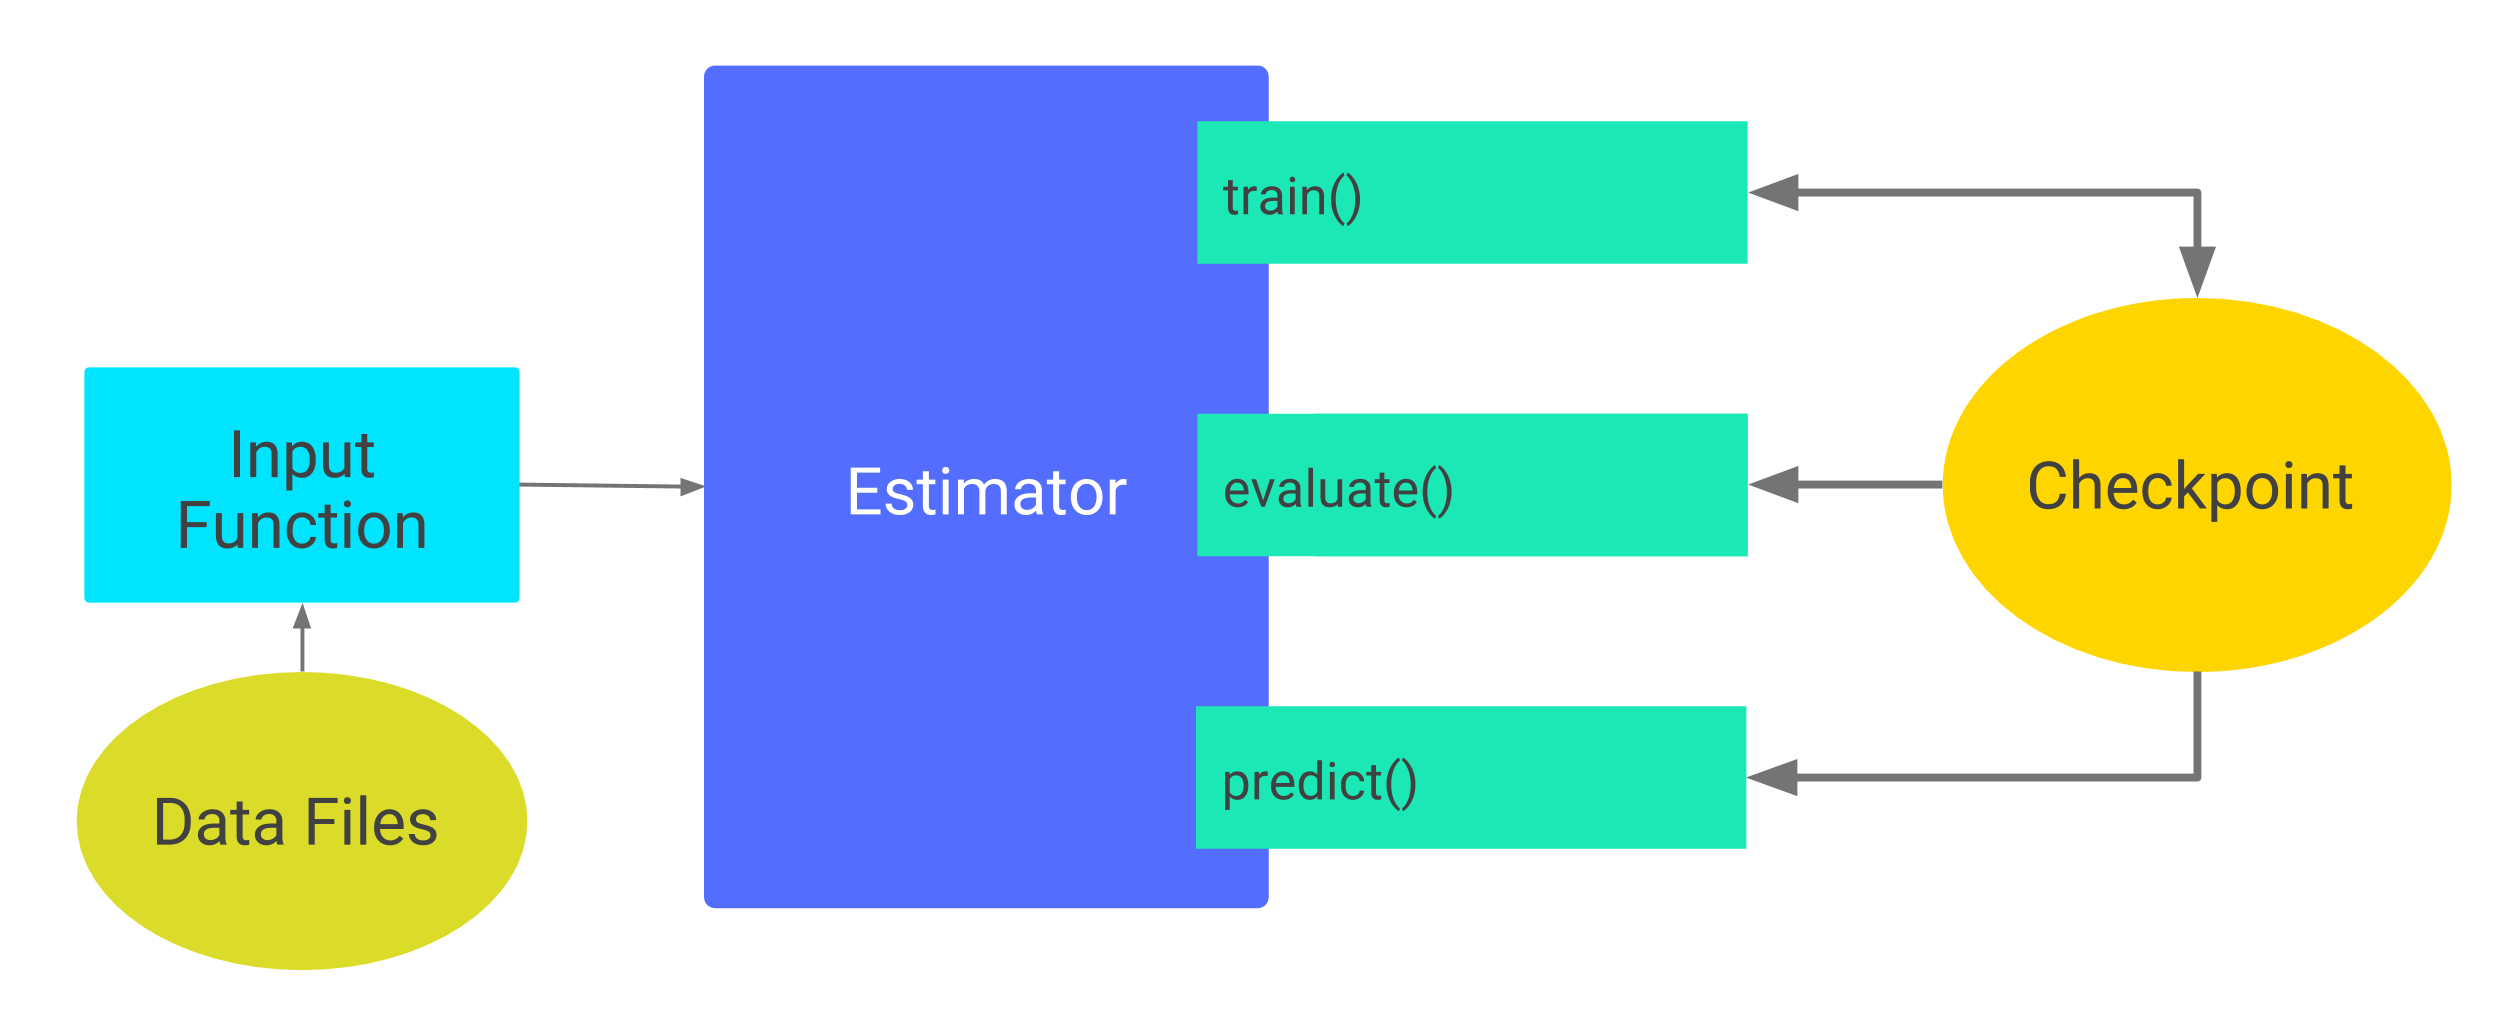
\includegraphics[height=6cm]{checkpoint.png}
  \captionof{figure}{Схема применения сериализациии и десериализации\cite{tf_doc:checkpoint}}\label{fig:func:checkpoint}
\end{center}

Так как поле \texttt{encoder} класса \texttt{cstlstm.ChildSumTreeLSTMClassifier} хранит ссылку на объект типа \texttt{cstlstm.ChildSumTreeLSTMCell}, но, при этом, объект типа \texttt{cstlstm.ChildSumTreeLSTMCell} может существовать независимо, то от класса \texttt{cstlstm.ChildSumTreeLSTMClassifier} направлена связь типа композиция в сторону класса \texttt{cstlstm.ChildSumTreeLSTMCell}. Данная композиция отображена на диаграмме классов, изображенной на чертеже ГУИР.400201.009.РР.1.

Класс \texttt{train.Treebank} контролируюет прогресс обработки некоторого набора данных. При создании объекта типа \texttt{train.Treebank} будет выгружен набор данных из базы данных или из файла. Затем, во время итерации по набору данных можно будет изображать прогресс выполнения с помощью вызова метода \texttt{print\_progress\_bar}. Данный метод будет рассчитывать текущий прогресс основываясь на публичном поле класса \texttt{train.Treebank} \texttt{size}, который хранит размер всего набора данных. Это необходимо, так как инструменты контроля набора данных в Tensorflow не поддерживают такой возможности. Так как класс \texttt{train.Treebank} используется при обработке набора данных классом \texttt{train.Train}, то от класса \texttt{train.Treebank} направлена связь типа ассоциация в сторону класса \texttt{train.Train}. Данная ассоциация отображена на диаграмме классов, изображенной на чертеже ГУИР.400201.009.РР.1. Код конструктора класса \texttt{train.Treebank} представлен ниже:
\medskip
\begin{lstlisting}[style=Python]
  def __init__(self, data_dir, set_name, embed_indexes):
    json_path = os.path.join(data_dir, 'json', set_name + '.json')
    set_path = os.path.join(data_dir, set_name)
    with codecs.open(json_path, encoding='utf-8') as f:
      trees = json.load(f)
    trees = [replace_words_by_index(tree, embed_indexes) for tree in trees]
    if set_name == 'train':
      trees = [tree for tree in trees if tree[0] != 2]
    self.size = len(trees)
    jsons = ''.join([json.dumps(tree) + '\n' for tree in trees])
    with open(set_path, 'w') as f:
      f.write(jsons)
    super(Treebank, self).__init__(set_path)
\end{lstlisting}
\medskip

Параметр конструктра \texttt{train.Treebank} \texttt{data\_dir} типа \texttt{str} --- путь к набору данных. Параметр \texttt{set\_name} типа \texttt{str} --- это название набора данных, которое будет отображаться в строке состояния. Параметр \texttt{embed\_indexes} типа \texttt{dict} --- это словарь соответствия слов индексам их векторов в матрице модели GloVe.

Класс \texttt{train.Train} контролирует процесс обучения модели Child-Sum Tree LSTM\@. Имеет следующие публичные поля:
\begin{itemize}
\item \texttt{epochs}
\item \texttt{learning\_rate}
\item \texttt{embedding\_learning\_rate}
\item \texttt{model}
\item \texttt{model\_optimizer}
\item \texttt{embedding\_optimizer}
\item \texttt{checkpoint}
\end{itemize}

Публичное поле \texttt{epochs} типа \texttt{int} класса \texttt{train.Train} хранит количество эпох обучения архитектуры Child-Sum Tree LSTM\@. За одну эпоху обучения модель обрабатывает весь тренировочный набор данных. Слишком низкое количество эпох может привести к недостаточному обучению модели. Слишком высокое, наоборот, может привести к переобучению. Либо же, если при оптимизации точность модели не будет сходиться, то большее количество эпох свыше какого-то порога сходимости не даст прироста производительности модели Child-Sum Tree LSTM\@. На рисунке~\ref{fig:func:epoches} показан пример зависимости ошибки нейронной сети от пройденных эпох обучения.

\begin{center}
  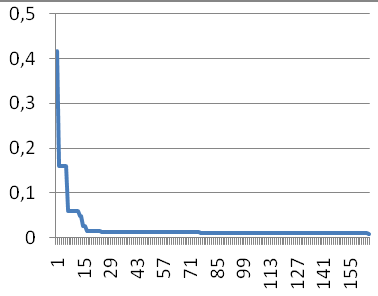
\includegraphics[height=6cm]{epoches.png}
  \captionof{figure}{Зависимость ошибки нейронной сети от количества пойденных эпох обучения\cite{Goodfellow-et-al-2016}.}\label{fig:func:epoches}
\end{center}

Публичное поле \texttt{learning\_rate} типа \texttt{float} класса \texttt{train.Train} хранит скорость обучения модели. Это коофициент в интервале [0, 1], который будет определять какая доля потери, вычислинной градиентным спуском, будет прибавлятся к тренируемым параметрам модели. На рисунке~\ref{fig:func:learning_rate} показаны зависимости ошибки от эпох обучения модели для разных скоростей обучения. Слишком низкая точность обучения может привести в тому, что модель может свестись только через черезмерно большое количество пройденных эпох обучения. Слишком большая скорость обучения может и вовсе привести к тому, что модель не сможет сойтись. Данный процесс изображен на рисунке~\ref{fig:func:learning_rate2}. Красной линией указана последовательность изменения весов модели нейронной сети.

\begin{center}
  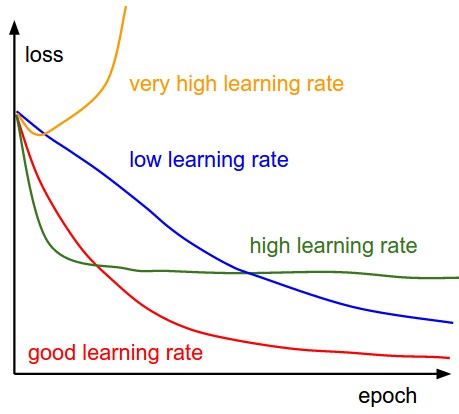
\includegraphics[height=6cm]{learning_rate.png}
  \captionof{figure}{Зависимость ошибки нейронной сети от количества пройденных этапов обучения, указанная для различных значений скорости обучения\cite{stanford_course}.}\label{fig:func:learning_rate}
\end{center}

\begin{center}
  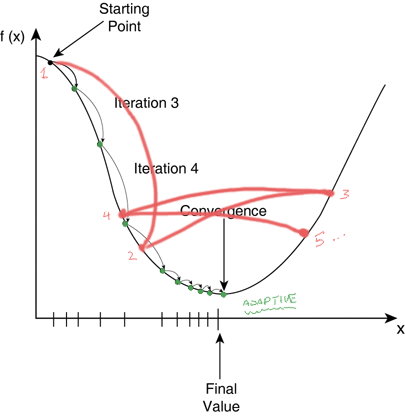
\includegraphics[height=6cm]{learning_rate2.png}
  \captionof{figure}{Сходимость функции потерь\cite{stanford_course}.}\label{fig:func:learning_rate2}
\end{center}

Публичное поле \texttt{embedding\_learning\_rate\_factor} типа \texttt{float} класса \texttt{train.Train} хранит коэффициент замедления скорости обучения слоя проекции встраивания слов. Так как при обучении модели происходит дообучение векторов модели GloVe, то, чтобы сохранить стабильность системы, необходимо использовать замедление скорости обучения. Замедляется встраивание слов, так как оригинальная модель GloVe обучалась без учителся на огромных наборах данных очень долгое время. Поэтому быстрое обучение на наборе из десяти тысяч синтаксических деревьев зависимотсей нарушит стабильность модели GloVe.

Класс \texttt{train.Train} имеет публичное поле \texttt{model} типа \texttt{cstlstm.Child\-SumTreeLSTMClassifier}, которое хранит ссылку на объект модели Child-Sum Tree LSTM\@. Данный объект модели и будет обучаться средствами \texttt{train.Tra\-in}.

Публичное поле \texttt{model\_optimizer} типа \texttt{tensorflow.AdagradOptimiz\-er} класса \texttt{train.Train} является имплементацией алгоритма Адаграда для оптимизации. Он будет применяться для оптимизации обучаемых весов всей модели.

Однако скорость обучения модели Child-Sum Tree LSTM и скорость обучения модели GloVe отличаются, и алгоритм оптимизации должен в разной степени влиять на веса в модели Child-Sum Tree LSTM и модели GloVe. Публичное поле \texttt{enbedding\_optimizer} типа \texttt{tensorflow.AdagradOptimizer} класса \texttt{train.Train} является имплементацией алгоритма оптимизации Ада\-града. Оптимизатор \texttt{model\_optimizer} применяется для следующих параметров:
\begin{itemize}
\item ядро слоя вычисления сигнала забывания Сhild-Sum Tree LSTM\@;
\item смещение слоя вычисления сигнала забывания Child-Sum Tree LSTM\@;
\item ядро слоя вычисления врат ячейки Child-Sum Tree LSTM\@;
\item смещение слоя вычисления врат ячейки Child-Sum Tree LSTM\@;
\item ядро слоя трансформации входов ячейки Child-Sum Tree LSTM\@;
\item смещение слоя вычисления трансформации входов ячейки Child-Sum Tree LSTM\@;
\item ядро логистической регрессии модели Child-Sum Tree LSTM\@;
\item смещение логистической регрессии модели Child-Sum Tree LSTM\@.
\end{itemize}
Оптимизатор \texttt{embed\_optimizer} применяется для следующих параметров:
\begin{itemize}
\item ядро плотного слоя проекции векторов GloVe модели Child-Sum Tree LSTM\@;
\item смещение плотного слоя проекции векторов GloVe модели Child-Sum Tree LSTM\@.
\end{itemize}

Публичное поле \texttt{checkpoint} типа \texttt{tensorflow.Checkpoint} класса \texttt{tra\-in.Train} является сериализатором модели Child-Sum Tree LSTM\@.

Класс \texttt{train.Train} хранит ссылку на объект класса \texttt{cstlstm.ChildSum\-TreeLSTMClassifier} и является независимым, поэтому от класса \texttt{train.Tra\-in} направлена связь типа агрегации в сторону класса \texttt{cstlstm.ChildSumTree\-LSTMClassifier}. Данная агрегация отображена на диаграмме классов, изображенной на чертеже ГУИР.400201.009.РР.1.

Ниже показан конструктор класса \texttt{train.Train}:
\medskip
\begin{lstlisting}[style=Python]
  def __init__(self, epochs, learning_rate, embedding_learning_rate_factor, checkpoint_dir, embed_dir):
    self.epochs = epochs
    self.learning_rate = learning_rate
    self.embedding_learning_rate_factor = embedding_learning_rate_factor

    embed, embed_indexes = self.load_embeddings(embed_dir)
    model = ChildSumTreeLSTMClassifier(embed)
    model_optimizer = tf.train.AdagradOptimizer(learning_rate)
    embedding_optimizer = tf.train.AdagradOptimizer(learning_rate * embedding_learning_rate_factor)
    checkpoint = model.checkpoint()
\end{lstlisting}
\medskip

Класс \texttt{train.Train} обладает следующими публичными методами:
\begin{itemize}
\item \texttt{replace\_words\_by\_index};
\item \texttt{train\_epoch};
\item \texttt{dev\_eval};
\item \texttt{evaluate\_dataset};
\item \texttt{load\_embedding}.
\end{itemize}

Публичный метод \texttt{replace\_words\_by\_index(tree, word2index)} класса \texttt{train.Train} заменяет слова в синтаксическом дереве зависимостей на индексы соответствующих им векторов в матрице отфильтрованных векторов GloVe. Данная операция необходима, чтобы во время обработки дерева воспользоваться средствами Tensorflow для загрузки плотных векторов.  Метдо получает параметр \texttt{tree} типа \texttt{list}, в котором хранится синтаксическое дерево зависимостей. Так же метод получает параметр \texttt{word2index} типа \texttt{dict}, где хранится соответствие слов из модели GloVe индексам их плотных векторов. Метод возвращает \texttt{list} в котором хранится исходное дерево, где слова заменены индексам векторов GloVe.

Публичный метод \texttt{train\_epoch} класса \texttt{train.Train} имеет следующие входные параметры:
\begin{itemize}
\item \texttt{model};
\item \texttt{train\_trees};
\item \texttt{model\_optimizer};
\item \texttt{embedding\_optimizer};
\item \texttt{batch\_size}.
\end{itemize}

Итак, метод \texttt{train\_epoch(model, train\_trees, model\_optimizer, embedding\_optimizer, batch\_size=25)} реализует эпоху обучения модели Child-Sum Tree LSTM\@. Параметр \texttt{model} типа \texttt{cstlstm.ChildSumTreeLSTMCla\-ssifier} хранит обучаемую модель Child-Sum Tree LSTM\@. Параметр \texttt{train\-\_trees} содержит тренировочный набор синтаксических деревьев зависимостей, которые хранятся в формате JSON\@, с заменнеными словами на индексы соответствующих им векторам GloVe. Параметр \texttt{model\_optimizer} типа \texttt{tensorflow.AdagradOptimizer} содержит имплементацию оптимизационного метода Адаграда для модели анализа тональностей в тексте Child-Sum Tree LSTM\@. Параметр \texttt{embedding\_optimizer} типа \texttt{tensorflow.AdagradOptimizer} содержит имплементацию оптимизационного метода Адаграда для модели встраивания слов GloVe. Параметр \texttt{batch\_size} содержит размер группы деревьев из набора данных. Тренировочный набор разбивается на группы в ходе тренировочной эпохи. После обработки каждой группы будет высчитываться градиент и оптимизироваться веса модели Child-Sum Tree LSTM\@. Размер группы --- это один из гиперпараметров модели. Большой размер группы ускорит эпоху обучения, так как количество групп, на которые поделен тренировочный набор равняется количеству оптимизаций модели, производимых за одну эпоху. Однако, чем меньше оптимизаций проводится, тем медленнее обучается модель, и при слишком большом размере группы оптимизатор будет делать слишком общие выводы для большого числа входных данных, а процесс обучения будет требовать большего количества эпох. При слишком маленьком размере группы время вычислений одной эпохи сильно возрастает, помимо этого оптимизатор будет длеать выводы на основе малого количества входных данных и модель будет подстраиваться под слишком индивидуальные особенности треднировочных данных, что может привести к переобучению. Влияение размера группы на процесс обучения отображено на рисунке~\ref{fig:func:batch_size}. Помимо примера большого и маленького размера группы, так же указан пример для случайного размера группы --- Stochastic Batch Size.

\begin{center}
  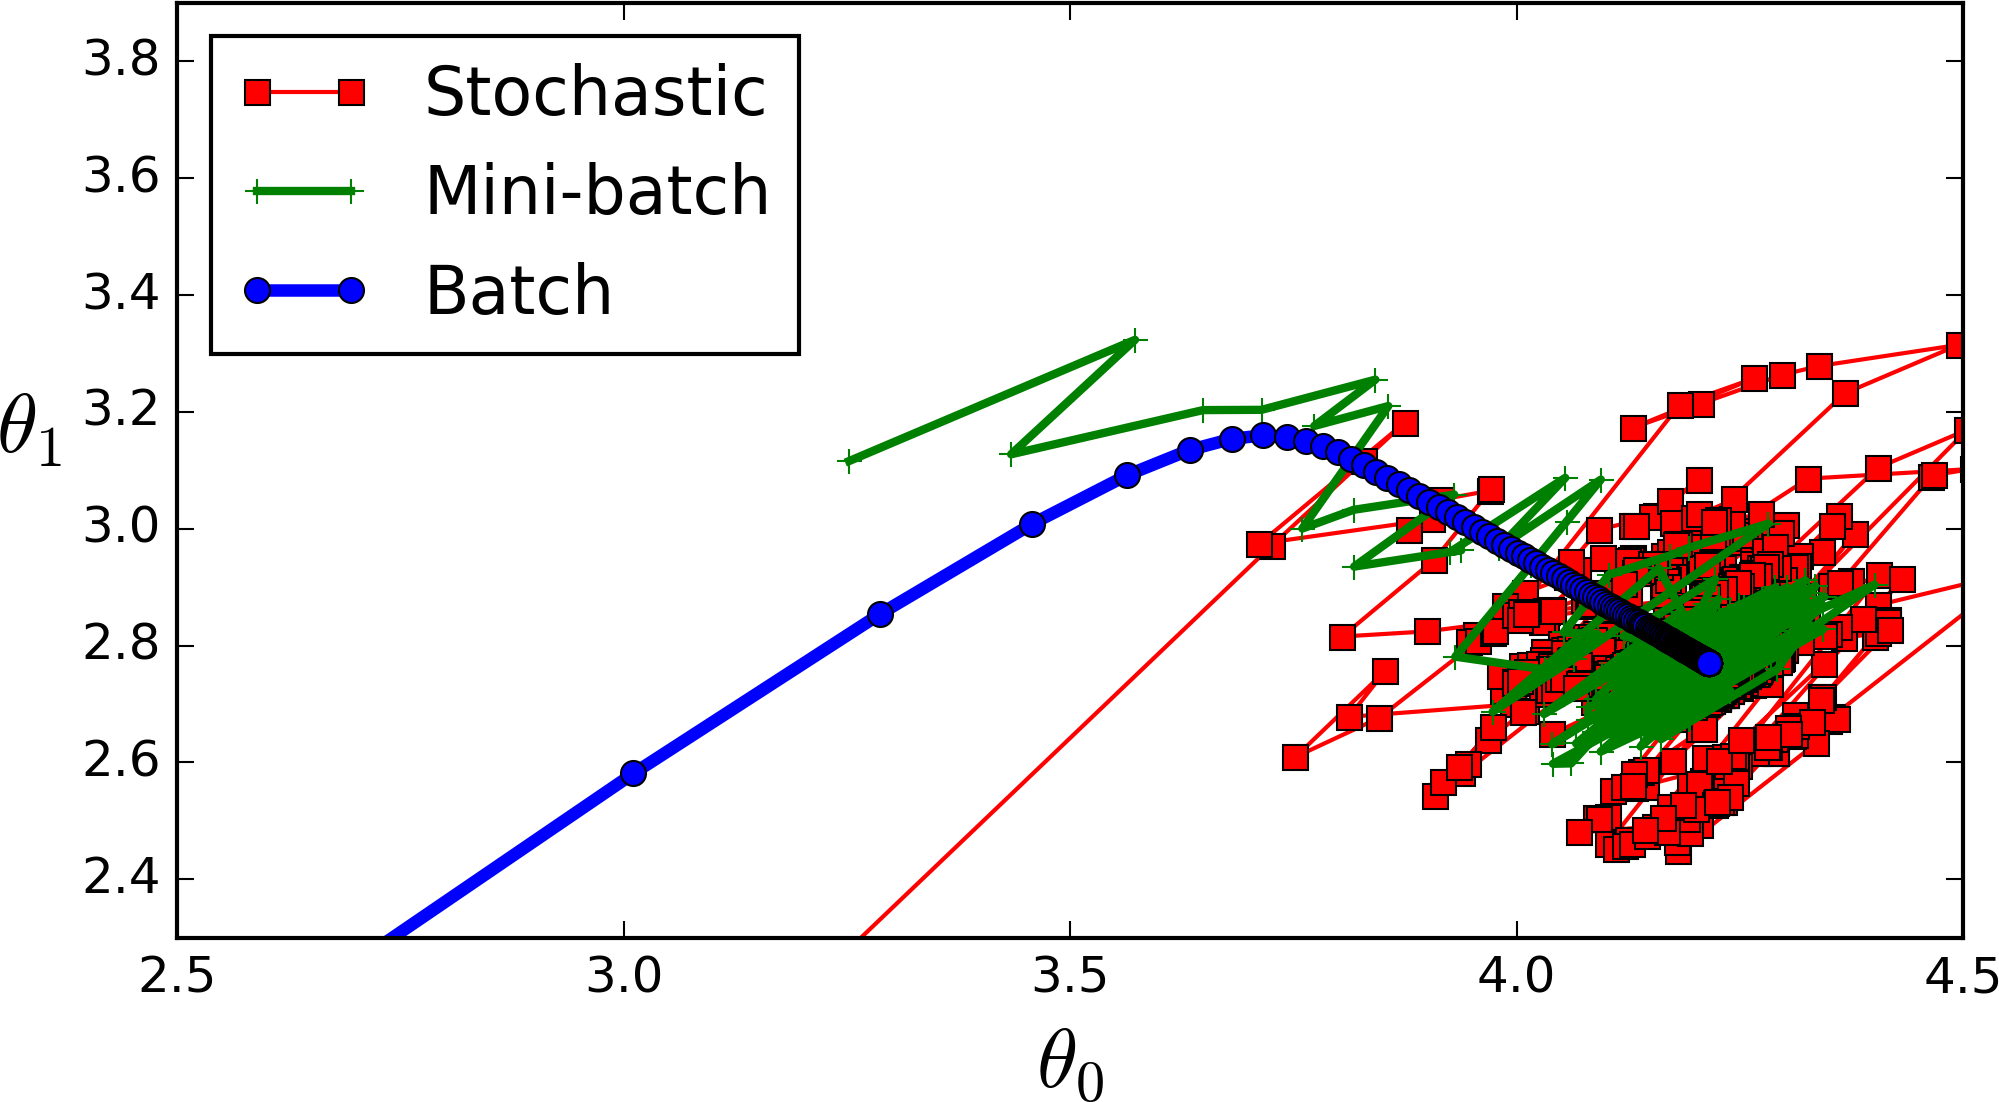
\includegraphics[height=6cm]{batch_size.png}
  \captionof{figure}{Влияение размера группы на процесс обучения\cite{stanford_course}.}\label{fig:func:batch_size}
\end{center}

Публичный метод \texttt{dev\_eval} класса \texttt{train.Train} имеет следующие входные параметры:
\begin{itemize}
\item \texttt{model};
\item \texttt{epoch};
\item \texttt{dev\_trees};
\item \texttt{train\_loss}.
\end{itemize}

Метод \texttt{dev\_eval(model, epoch, dev\_trees, train\_loss)} реализует обработку набора данных dev, который предназначен для настройки гиперпараметров модели. Так как гиперпараметры настраиваются специалистом на основе результатов работы системы, то метод \texttt{dev\_eval} просто выводит всевозможные метрики и информацию о ошибках модели. Пареметр \texttt{model} типа \texttt{cstlstm.ChildSumTreeLSTMClassifier} хранит обучаемую модель Child-Sum Tree LSTM\@ Параметр \texttt{epoch} типа \texttt{int} хранит номер этохи обучения. В параметре \texttt{dev\_trees} типа \texttt{list} хранятся синтаксические деревья зависимостей, сохраненные в json фомате. Параметр \texttt{train\_loss} типа \texttt{float} хранит значение функции потерь модели за текущую эпоху обучения.

Публичный метод \texttt{evaluate\_dataset(model, trees, batch\_size=25)} класса \texttt{train.Train} реализует обработку набора данных синтаксических деревьев зависимостей. Пареметр \texttt{model} типа \texttt{cstlstm.ChildSumTreeLSTMCla\-ssifier} хранит обучаемую модель Child-Sum Tree LSTM\@. В параметре \texttt{trees} типа \texttt{list} хранятся синтаксические деревья зависимостей, сохраненные в json фомате. Параметр \texttt{batch\_size} содержит размер группы деревьев из набора данных. Набор синтаксических деревьев зависимостей разбивается на группы в ходе обработке набора, и модель выполняется для всех деревьев одной группы одновременно. Метод возвращает средние значения точности для:
\begin{itemize}
\item классификации на 5 классов для корневых узлов деревьев;
\item классификации на 5 классов для всех узлов деревьев;
\item бинарной классификации на для корневых узлов деревьев;
\item бинарной классификации на для всех узлов деревьев.
\end{itemize}

Класс \texttt{train.Train} владеет публичным методом \texttt{load\_embeddings(em
  -bedding\_path)}, который реализует загрузку модели встаивания слов GloVe. Единственный входной параметр \texttt{embedding\_path} типа \texttt{str} хранит путь к модели GloVe. Метод возвращает матрицу типа \texttt{tensorflow.Tensor}, где хранятся плотные векторы слов, и словарь типа \texttt{dict}, который хранит соответсвие слов индексам их плотных векторов в матрице модели GloVe.

Класс \texttt{inference.Inference} управляет процессом предсказаний с помощью обученной модели Child-Sum Tree LSTM\@. Имеет следующие публичные поля:
\begin{itemize}
\item \texttt{model};
\item \texttt{tree};
\item \texttt{result};
\item \texttt{pretty\_tree}.
\end{itemize}

Код конструктора класса \texttt{inference.Inference} показан ниже:

\medskip
\begin{lstlisting}[style=Python]
  def __init__(self, path_to_jar, path_to_models_jar, sentence, embed_path, checkpoint_path):
    dependency_parser = StanfordDependencyParser(path_to_jar=path_to_jar, path_to_models_jar=path_to_models_jar)
    tokens = nltk.word_tokenize(sentence)
    tree = dependency_parser.parse_one(tokens)
    tree = tree.tree()

    embed, embed_indexes = load_embeddings('./data/filtered_glove.txt')
    self.model = ChildSumTreeLSTMClassifier(embed)
    checkpoint = model.checkpoint()
    checkpoint.restore(tf.train.latest_checkpoint(checkpoint_directory))
    self.tree = json.dumps(tree_to_list(tree, embed_indexes))
    self.result = []
    self.pretty_tree = None
\end{lstlisting}
\medskip

Входные параметра конструктора \texttt{inference.Inference}:
\begin{itemize}
\item \texttt{path\_to\_jar};
\item \texttt{path\_to\_directory};
\item \texttt{sentence};
\item \texttt{embed\_path};
\item \texttt{checkpoint\_path}.
\end{itemize}

Параметр \texttt{path\_to\_jar} типа \texttt{str} хранит путь к программе синтаксического анализатора CoreNLP\@. Парметр \texttt{path\_to\_models\_jar} типа \texttt{str} задает путь к модели shift reduce синтаксического анализатора зависимостей. Параметром \texttt{sentence} типа \texttt{str} задается предложение, которое необходимо обработать. Параметр \texttt{embed\_path} типа \texttt{str} хранит путь к модели встраивания слов GloVe. Параметр \texttt{checkpoint\_path} типа \texttt{str} хранит путь к модели Child-Sum Tree LSTM\@.

Публичное поле \texttt{model} класса \texttt{inference.Inference} типа \texttt{cstlstm.Ch\-ildSumTreeLSTMClassifier} хранит модель Child-Sum Tree LSTM\@. Так как класс \texttt{inference.Inference} хранит ссылку на объект класса \texttt{cstlstm.Child\-SumTreeLSTMClassifier}, однако, при удалении объекта модели, объект предсказателя дожен сохраняться, то от класса \texttt{inference.Inference} направлена связь типа агрегация в сторону класса \texttt{cstlstm.ChildSumTreeLSTMClassifi\-er}. Данная агрегация отображена на диаграмме классов на чертеже ГУИР. 400201.009.РР.1.

Публичное поле \texttt{tree} класса \texttt{inference.Inference} типа \texttt{str} хранит синтаксическое дерево зависимостей анализируемого предложения в формате JSON\@.

Публичное поле \texttt{result} класса \texttt{inference.Inference} типа \texttt{int[]} хранит результаты аналзиа тональностей дерева для каждого узла синтаксического дерева зависимостей. Результаты предсказаний храняться в развертке, в последовательности соответствующей порядку обхода дерева методо поиска в глубину.

Публичное поле \texttt{pretty\_tree} класса \texttt{inference.Inference} типа \texttt{visu\-alization.LabeledTree} хранит ссылку на объект дерева, подлежащего визуализации с помощью \texttt{visualization.Visualizator}. Так как предсказатель может существовать независимо от дерева визуализации, то от класса \texttt{infer\-ence.Inference} направлена связь типа агрегация в сторону класса \texttt{visuali\-zation.LabeledTree}. Данная агрегация отображена на диаграмме классов на чертеже ГУИР.400201.009.РР.1.

Класс \texttt{inference.Inference} обладает следующими публичными методами:
\begin{itemize}
\item \texttt{tree\_to\_list(tree, embed\_indexes)};
\item \texttt{load\_embeddings(embedding\_path)};
\item \texttt{convert\_result(tree, results)}.
\end{itemize}

Публичный метод \texttt{tree\_to\_list(tree, embed\_indexes)} класса \texttt{infe\-rence.Inference} преобразует дерево из формата, возращаемого синтаксическим анализатором CoreNLP в входной формат модели Child-Sum Tree LSTM\@. Параметр \texttt{tree} типа \texttt{nltk.Tree} хранит дерево в фомате CoreNLP\@. Параметр \texttt{embed\_indexes} типа \texttt{dict} сранит словарь соответствий слов их плотным векторам в модели GloVe.

Публичный метод \texttt{load\_embeddings(embedding\_path)} класса \texttt{infere\-nce.Inference} реализует загрузку модели встаивания слов GloVe. Единств\-енный входной параметр \texttt{embedding\_path} типа \texttt{str} хранит путь к модели GloVe. Класс \texttt{train.Train} преобразует модель GloVe к тензору Tensorflow, но в реализации этого метода класса \texttt{Inference} нет необходимости в поиске плотных векторов слов во время выполнения модели Child-Sum Tree LSTM, так как предсказатель работает только с одинм деревом.

Публичный метод \texttt{convert\_result(tree, results)} класса \texttt{Inference} преобразует синтаксическое дерево зависимостей в формат, пригодный для визуализации. Параметр \texttt{tree} типа \texttt{list} хранит дерево в формате модели Child-Sum Tree LSTM\@. Параметр \texttt{results} хранит результаты работы системы анализа тональностей в последовательности обхода синтаксического дерева методом поиска в глубину. Метод \texttt{convert\_result(tree, results)} возвращает дерево в пригодном для визуализации формате типа \texttt{visualization.La\-beledTree}.

\subsection{Модуль визуализации TensorBoard}
Модуль визуализации TensorBoard представляет собой отдельно приложение, которое визуализирует внутренние процессы, протекающие в модели машинного обучения. Поэтому этот модуль визуализации не имеет представления на диаграмме классов. В код проекта он ключен только в виде специальных меток, позволяющий TensorBoard собирать информацию о модели.

\subsection{Модуль визуализации CoreNLP}
Модуль визуализации CoreNLP выводит синтаксическое дерево зависимостей обработанного предложения и демонстрирует последовательность, в которой модель Child-Sum Tree LSTM делала выводы. Модуль представлен двумя классами:
\begin{itemize}
\item \texttt{visualization.LabeledTree};
\item \texttt{visualization.Visualizator}.
\end{itemize}

Класс \texttt{visualization.LabeledTree} представляет синтаксическое дерево зависимостей с предсказанными уровнями тональностей для кахдой фразы в предложении. Класс имеет следующие публичные поля:
\begin{itemize}
\item \texttt{label};
\item \texttt{children};
\item \texttt{text};
\item \texttt{parent};
\item \texttt{depth}.
\end{itemize}

Публичное поле \texttt{label} типа \texttt{int} класса \texttt{visualization.LabeledTree} содержит значение тональности для данного дерева. Поле \texttt{children} типа \texttt{vi\-sualization.LabeledTree[]} хранит ссылки на объекты данного класса, которые являются детьми текущего объекта. Поле \texttt{parent} типа \texttt{visualizati\-on.LabeledTree} содержит ссылку ссылку на объект узла-родителя текущего дерева. Таким образом содается древовидная структура, каждый узел которой является объектом класса \texttt{visualization.LabeledTree}. Поле \texttt{text} типа \texttt{str} хранит слово или фразу, соответствующее текущему узлу. Поле \texttt{depth} типа \texttt{int} хранит глубину текущего дерева. Это необходимо для операций нормализации дерева.

Код конструктора класса \texttt{visualization.LabeledTree} предствлен ниже:
\medskip
\begin{lstlisting}[style=Python]
    def __init__(self, depth=0, text=None, label=None, children=None, parent=None):
        self.label    = label
        self.children = children if children != None else []
        self.general_children = []
        self.text = text
        self.parent   = parent
        self.depth    = depth
\end{lstlisting}
\medskip

Публичный метод \texttt{add\_child(child)} класса \texttt{visualization.Labeled\-Tree} добваляет узел в список детей текущего узла. Параметр \texttt{child} типа \texttt{vi\-sualization.LabeledTree} хранит объект дерева, которое будет добавлено в список детей.

Публичный метод \texttt{to\_dict()} класса \texttt{visualization.LabeledTree} преобразует текущее дерево в словарь, который хранит всю необходимую информацию и позволяет воссоздать дерево из солваря без потери информации. Метод возвращает объект типа \texttt{dict}.

Публичный метод \texttt{to\_json()} класса \texttt{visualization.LabeledTree} сериализует текущее дерево в формат JSON. Метод возвращает объект типа \texttt{str}.